
%
\documentclass[%
 reprint,
 amsmath,amssymb,
 aps,
]{revtex4-1}

\usepackage{graphicx}% Include figure files
\usepackage{dcolumn}% Align table columns on decimal point
\usepackage{bm}% bold math


\begin{document}

\title{Sistema de Gestion para el concurso de Proyectos de la EPIS}
\author{Jose Pastor Mendoza}
\author{Franklin Huichi Contreras}
\author{Andrés De La Barra Vasquez}
\affiliation{%
 Universidad Privada de Tacna \textbackslash Facultad de Ingenieria \textbackslash Escuela Profesional de Ingenieria de Sistemas
}%

\begin{abstract}
\begin{center}
\textbf{Resumen}
\end{center}
Debido a que se usan diferentes herramientas durante la gestión del concurso de proyectos de Escuela Profesional de Ingeniería de Sistemas de la Universidad Privada de Tacna, se desarollará un sistema web denominado "Sistema de Administracion de Proyectos para la EPIS" donde se pueda realizar la gestión y unificar los procesos que conlleva el concurso de proyectos.


\begin{center}
\textbf{Abstract}
\end{center}
Due to the fact that different tools are used during the management of the project contest of the Professional School of Systems Engineering of the Private University of Tacna, a web system called "Project Management System for EPIS" will be developed where the management can be carried out. and unifying the processes involved in the competition for projects.

\end{abstract}



\maketitle

%\tableofcontents

\section {Introducción}

Los sistemas de gestion es un metodo que se usa para poder administrar, dirigir, operar y observar los cambios de una empresa, institucion, o una area determinada con el fin de poder generar resultados positivos y toma de decisiones basadas en datos o hechos concretos. El sistema de gestion a su vez permite tener eficiencia y eficacia en desempeño de una organizacion inlcuyendo calidad en la misma gestion del area objetivo.\\
Es por ello que en el presente proyecto va referido al rubro de educación universitaria; ya que se observó que en la Escuela Profesional de Ingeniería de Sistemas realizan algunos procesos de manera no automatizada para la gestión del concurso de proyectos, debido a ello este proyecto se justifica para el beneficio del concurso y la insticuion la cual implica a los estudiantes, administradores y jurados.

\section{Autores}
\begin{itemize}
\item José Edilberto Pastor Mendoza.
\item Franklin Carlos  Huichi Contreras.
\item Andrés De La Barra Vasquez.
\end{itemize}

\section{Planteamiento del problema}
\subsection{Descripcion del problema}
En la Universidad Privada de Tacna con referencia al concurso de proyectos de la misma institucion no cuenta con una estructura definida en los concursos liberados durante el semestre academico. \\
Los problemas que se encontro son los siguientes:
\begin{itemize}
\item Los docentes para asegurar la calidad del concurso nesecitan revisar que el proyecto no se haya realizado anteriormente, es por ello que se basan en el historial de los proyectos presentados en anterioridad, para ello realizan esta revision en conjunto con la documentacion presentada por los alumnos no sea una copia de documentos de proyectos anteriormente presentados en el concurso para ello realizan una comparacion con la documentacion de proyectos anteriores haciendo de este una tarea tediosa y casi imposible de poder abarcar todas las documentaciones presentadas.
\item  Por parte del alumnos tambien el problema seria de que al no saber como se presenta  una documentacion adecuada sufre constantes problemas al momento de entregar, debido a que resulta que no tiene el formato adecuado la documentacion presentada al docente. 
\item Otro problema que se observo y que muchos alumnos demandaban era la transparencia en los votos realizados durante el concurso de proyectos, lo cual ellos querian saber en que criterio de calificacion fallaron segun los jurados, en la cual los estudiantes tambien querian votar por sus proyectos favoritos de manera que esten involucrados como parte de este concurso.
\item Otro problema que se observo es que debido a la gran cantidad de proyectos presentados anteriormente existe ideas parecidas o iguales ya realizadas, esto hace que los alumnos al desconocer la existencia de estos proyectos repiten los mismos haciendo los concursos monotonos y con falta de originalidad.
\end{itemize}

\subsection{Problema}
\subsubsection{General}
¿ Podra un sistema de gestion resolver los problemas del concurso de proyectos?
\subsubsection{Especificos}
\begin{itemize}
\item ¿Podra el sistema resolver el problema de los alumnos acerca de la correcta presentacion de la documentacion del proyecto?
\item ¿El sistema podra detectar si el documento de un alumno es realizado de manera legal y que no contiene copia alguna de documentacion anteriormente presentadas ?
\item ¿El sistema podra tener transpariencia en su votacion en el transcurso del concurso de proyectos ?
\end{itemize}
\subsection{Justificacion}
Hoy en día las empresas necesitan tecnologia para que sus empleados sean eficientes en su trabajo, de esta manera pueden beneficiarce para obtener una mejor calidad de servicio, mejorar sus procesos y por consiguiente clientes satisfechos.

\subsection{Alcance}
El proyecto se realizara para la gestion de concursos de proyectos en la escuela de la epis, que tendran los modulos de revision, sorteo, categorias, cursos, docentes, creacion de eventos y el seguimiento de votos para la gestion de el concurso de proyectos. 

%-----------------------------------------------------------------
\section {Objetivos}
\subsection {General}
Resolver los problemas del concurso de proyectos aplicando tecnologias de parte web y movil. Asu vez integrar todas las actividades involucradas en el proceso del concurso de proyectos ,explicados como problemas, de la EPIS.
\subsection {Especificos}
\begin{itemize}
\item Crear un servicio que nos permita verificar si un documento es unico y no una copia del historial de documentos.
\item Crear un servicio que nos permita subir los proyectos a una base de datos.
\item Crear un servicio que nos permita autenticar nuestras credenciales en una base de datos.
\item Integrar estos servicios en una aplicacion movil y en un sitio web, todo ello haciendo el uso correcto que nesecite cada una de las aplicaciones.
\end{itemize}

\section {Desarrollo de la propuesta}
La siguiente propuesta cuenta con tres puntos :
\begin{itemize}
\item Realizar una aplicacion web donde los alumnos tendran disponible un repositorio con toda la informacion sobre los proyectos presentados en ciclos pasados y un formulario donde podran registrarse los proyectos que van a participar del concurso. Ademas la aplicacion web tendra otra vista unica para el administrador del sistema, el cual se encargara de revisar los proyectos inscritos que tengan advertencia de plageo, agregara categorias, cursos, asignara docentes al concurso, ademas de poder visualizar el reporte de votos.  
\item Realizaremos un servicio que detecte si los documentos cumplen con la plantilla establecida parar la inscripcion al concurso, ademas de tener un detector de plageas comparando con datos historicos.
\item Relizaremos una aplicacion movil para que los jurados puedan votar.
\end{itemize}
\newpage
Tecnologias que usaremos :
\begin{itemize}
\item Nodejs
\item Reactjs
\item Python
\item MongoDB
\item Firebase
\end{itemize}
\begin{center}
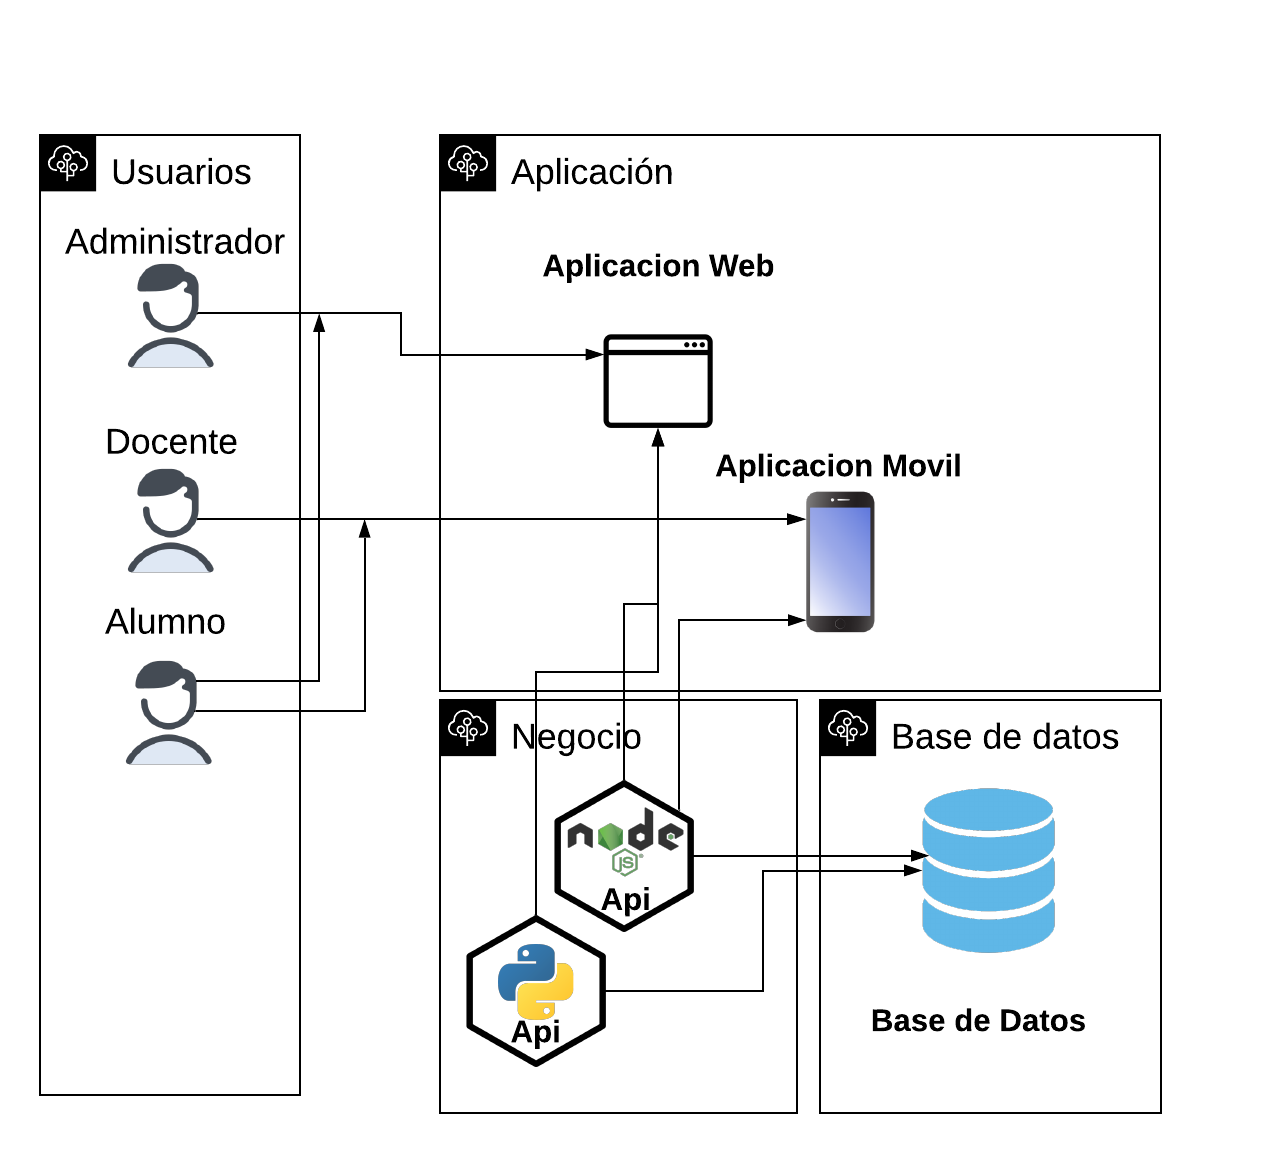
\includegraphics[width=10cm]{./Imagenes/arquitectura2}
\end{center}

%-----------------------------------------------------------------
\section{Conclusiones}

\begin{itemize}
\item La presente propuesta resuelve e integra las actividades totales que conlleva la realización del concurso de proyectos de la EPIS, tales como la inscripción de los participantes, organización de los equipos y también calificación de los jurados. 

\item La implentacion de una funcionalidad extra, que es la posibilidad de los estudiantes espectadores  para votar por el proyecto que más simpatizan,  solicitada por la organizadora del concurso como una posibilidad a implementar a futuro. 

\item Las tecnologías web a aprender y desarrollar durante el proceso del proyecto involucran la actualización e investigación por parte del grupo de trabajo, lo cual cumple uno de los objetivos principales como estudiantes de la carrera de Ingenieria de Sistemas, el cual es ser autodidactas y buscar la constante capacitacion, al tener tecnologias renovadas cada dia.
 

\end{itemize}

% Bibliografia.
%-----------------------------------------------------------------

%\bibliographystyle{plain}
%\bibliography{Bibliografia}

\end{document}

